\documentclass[tikz,border=10pt]{standalone}
\usepackage{tkz-euclide} % 强化几何作图

\begin{document}
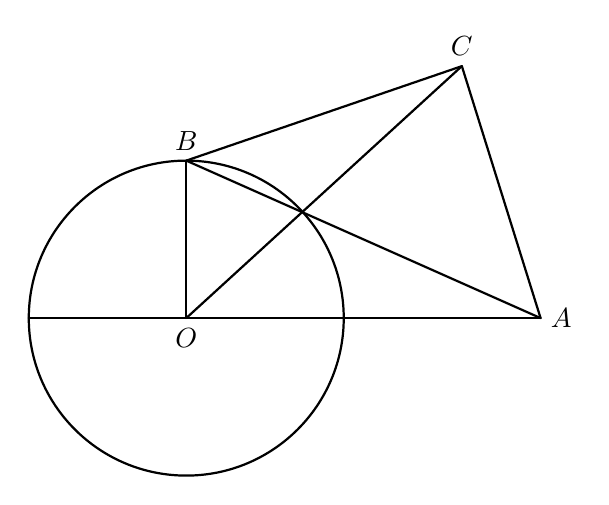
\begin{tikzpicture}[line join=round, line cap=round, >=stealth, thick]

    % 1. 定义基本参数
    \def\r{2}    % 圆的半径
    \def\ax{4.5} % 点A的横坐标
    \def\cx{3.5} % 点C的横坐标
    \def\cy{3.2} % 点C的纵坐标

    % 2. 定义坐标点
    \coordinate (O) at (0,0);
    \coordinate (B) at (0,\r);
    \coordinate (A) at (\ax,0);
    \coordinate (C) at (\cx,\cy);
    \coordinate (L) at (-\r,0); % 圆左侧的直径端点

    % 3. 绘制圆形
    \draw (O) circle (\r);

    % 4. 绘制所有实线连接
    \draw (L) -- (A);          % 水平直径及延长线
    \draw (O) -- (B);          % 半径 OB
    \draw (O) -- (C);          % 连线 OC
    \draw (B) -- (C);          % 连线 BC
    \draw (C) -- (A);          % 连线 CA
    \draw (B) -- (A);          % 连线 BA (对角线)

    % 5. 标注点名称
    % anchor 用于微调文字与点之间的距离和方向
    \node at (O) [below] {$O$};
    \node at (B) [above] {$B$};
    \node at (A) [right] {$A$};
    \node at (C) [above] {$C$};

    % 6. (可选) 如果需要强调直角，可以使用 tkz-euclide 标注
    % \tkzMarkRightAngle[size=0.2](B,O,A)

\end{tikzpicture}
\end{document}